\chapter{\label{app2:theory}Appendix: A general account of team click in group exercise}

\begin{CJK}{UTF8}{gbsn}



\section{Active inference framework}

\subsection{Predictive Coding\label{app2:predictiveCoding}}
PC first emerged as a data processing and compression strategy in computer science \citep{Rao1999}.  Researchers programmed a multi-layer artificial neural network to use downwards connections to match samples of .JPEG images with successful predictions. Visual signals were processed via a hierarchical system in which each level tried to predict activity at the level below it using recurrent feedback connections. If the feedback successfully predicted the lower-level activity, no further action was required. Failure of the model to predict the visual signal resulted in tuning and revision of the model using ``residual errors'' derived from the discrepancy between top-down predictions and lower-level activity.  Predictive coding offered a much more computationally efficient mechanism for data processing than previous alternatives, because prediction errors were the only informational novelties in the system \citep{Clark2015}.

\subsection{Motor control\label{app2:motorControl}}
Successful regulation with the environment depends on an organism's capacity to move from its current state to a desired state.  In the case of the human evolutionary niche, organismic regulation hinges largely on movement, be it physical or simulated \citep{Wolpert1995}.

Theories of motor control generally agree the brain generates ``forward models'' that anticipate perceptual inputs and desired motor states \citep{Pickering2014}. The first paradigmatic theory of motor control suggested that forward models for action relied on special-purpose mechanism auxiliary to core mechanisms of perception of action \citep{Wolpert1997}.  This hypothesis, now known as the Auxiliary Forward Model \citep[AFM, see][]{Pickering2014}, relies on a dual mechanism of motor control.  First, a motor command is estimated in the brain by an ``inverse model,'' which contains as its inputs both the desired state and the actual state of the organism (e.g., the position of the body, see Figure ~\ref{fig:AFM}).  When the motor command is generated, an auxiliary copy (i.e., an ``efference copy'') is also generated, and is sent to a forward model which then generates predictions about action and perception by simulating the musculoskeletal system and contextual environment \citep{Wolpert1995,Blakemore1998,Flanagan2003}.  Prediction error arising from a discrepancy between predicted and resultant sensory inputs are then used as feedback to inform the generation of the next motor command in the inverse model, and so on in a loop, until the fit between sensory prediction and input is sharpened.

A more recent alternative proposal to the AFM suggests that forward models, instead of being auxiliary to, may instead lie at the heart of all forms of perception and action \citep{Friston2010}.  In contrast to AFM, the ``Integrative Forward Models'' account of motor control \citep[IFM, see][]{Pickering2014} posits that predictions from forward models act directly as action commands.  There is no dedicated mechanism used to predict the outcomes of our own (or others') actions in addition to the action commands themselves.  Instead, generative action-oriented models are treated as the actual state of affairs, and cause a cascade of downward predictions about what should be the state of the models in the levels below (see Figure ~\ref{fig:IFM}).  In the IFM approach, there is no need for a motor command or efference copy at each level of action prediction, and prediction errors directly update the action models themselves.


\begin{figure}[htbp]
  \begin{center}
    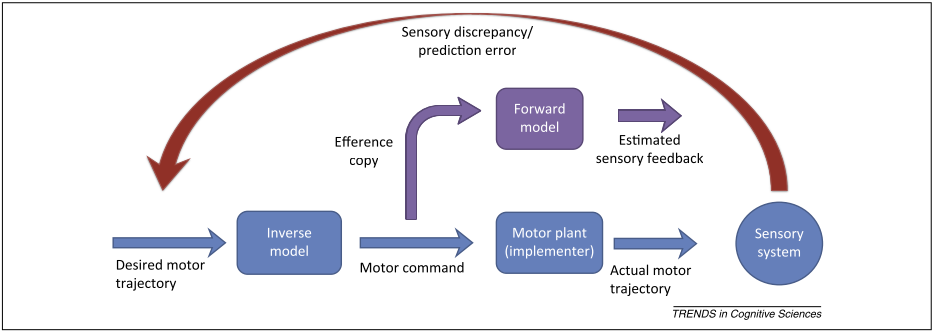
\includegraphics[scale=.3]{images/AFM.png}
      \caption{The Auxiliary Forward Model of motor control}
        \label{fig:AFM}
   \end{center}
\end{figure}

\begin{figure}[htbp]
  \begin{center}
    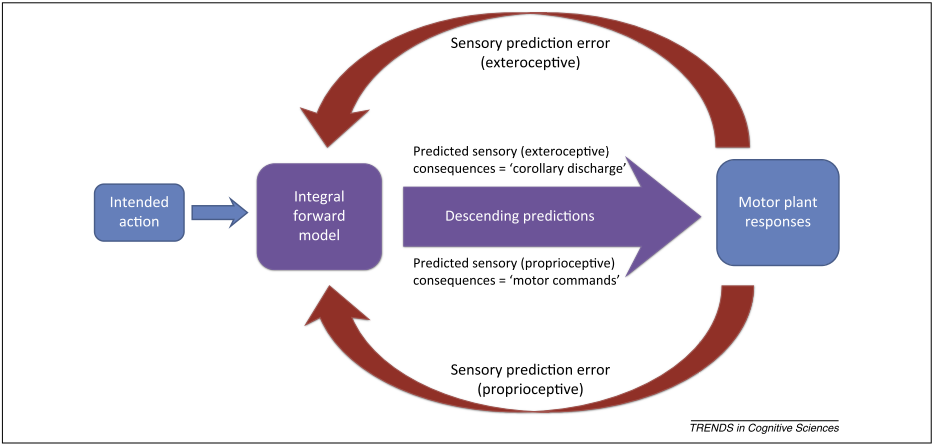
\includegraphics[scale=.3]{images/IFM.png}
      \caption{The Integrated Forward Model of motor control}
        \label{fig:IFM}
   \end{center}
\end{figure}


Both the AFM and IFM approaches agree that prediction, error minimisation, and hierarchical modelling are core processes in human cognition. From a thermodynamic standpoint, however, IFM appears to offer a more efficient model for free energy minimisation.  By replacing motor commands with direct predictions about proprioceptive and exteroceptive consequences, the need for a distinct optimal control calculation (i.e. an inverse model) disappears and along with it the need for an efference copy of the motor command, thus implicitly minimising various energetic costs \citep{Pickering2014,Friston2010}.   In place of the auxiliary mechanisms of the AFM, IFM posit a more complex (distributed) forward model mapping prior beliefs about desired trajectories to sensory consequences.  Whereas the ``heavy lifting'' in AFM required the use of an efference copy and inverse models, in IFM this work is done by the acquisition and use of a more complex predictive (generative) model \citep{Pickering2014}.

%, which appear to be maximised in team click.



\subsubsection{AFM approach to joint action\label{app2:AFMapproachJA}}
 \textcite{Keller2016}, for example, presented a conceptual framework that applies an ``auxiliary forward model'' (AFM) approach to musical joint actions.  The AFM approach requires that agents produce models responsible for 1) individual action planning and control (self-internal models), 2) prediction of others' actions (other-internal models), and 3) representation of the shared goal (joint-internal models).  Of these three types of models, however, only self-internal models comprise the auxiliary predictive architecture (i.e., the forward model containing an efference copy of one's own action, and ``inverse models'' that are responsible for output of motor commands.  Thus, both anticipation and compensation in joint action depends on a control loop, whereby sensory information (error signals) are routed (fed-back) through self-internal models, which inform the production of auxiliary predictions---of self, other, and joint action---grounded in individual motor simulations.  Importantly, in this model,  error signals are fed-back only to the self-inverse model, as no inverse model for the joint action partner exists.
 %See Appendix~\ref{app2:motorControl} for a more detailed explanation of these terms).

The now longstanding proposal that individuals only produce auxiliary predictive models of their own actions (as opposed to others' actions too) has served to explain how individuals effectively attend to others in joint action.  With privileged access to an efferent copy of impending individual action, an agent is able to preemptively attenuate sensitivity to their own action, in order to attend to the actions (and prediction errors) of others \citep{Wolpert1998}.  For example, the AFM approach provides an explanation for the phenomenon of tickling, or specifically why it is near impossible to tickle oneself \citep[due to sensory attenuation resulting from the self-generated predictions about the consequences of action][]{Blakemore2003}. However, while the AFM has proven adequate to explain individual motor control, and some instances of joint action (such as tickling), it also contains potential shortcomings when applied to dynamical joint action scenarios.

\textcite{Pesquita2017} summarise three shortcomings of an AFM approach to joint action.  First, the AFM model assumes a static and unchanging representation of the shared goal and the other's goal, and provides no mechanism through which the shared goal representation can be dynamically updated (based on prediction error signals).  This issue limits the ability of AFM to account for the real-world flexibility and interchangeability of shared goals (for example, the adaptive switching between the shared goal of carrying a table or the bench depending on the location of both objects).  Second, the same rigidity applies to other-inverse models.  The inability to directly and dynamically update other-models suggests the practical possibility that self and other models may gradually diverge over time due to the lack of sufficient predictive information regarding the actions of others \citep{Pickering2014}. Third, the AFM approach does not specify how sensory input is differentially used to update self and other models, which limits the model's ability to account for learning and adaptation within joint action \citep{Pesquita2017}.  Thus, not only does the AFM approach appear to be computationally intensive (due to the recruitment of auxiliary inverse models and dual motor commands, it also appears to be unable to fully account for the dynamic interactive flexibility required of agents in real-world joint action.

%\myparagraph{Generalised synchronisation as a dynamical foundation for joint action}

\myparagraph{Precision-weighting self- and others}
In place of auxiliary processes of prediction, the AIF for joint action hinges instead on precision weighting of prediction errors in order to facilitate and finesse joint action \citep{Friston2015,Friston2015a}.  When engaged in joint action, the individual turns down the volume (reduce the precision weighting) on prediction errors relating to one's own action so that movement can occur unimpeded by over-attention to self-generated prediction errors \citep[an intuitive example of the opposite of this ideal scenario is a Skype call in which the flow of an individual's speech is interrupted by auditory feedback from the other receiver's device (feedback that would otherwise be attenuated by the speaker), see][]{Friston2015}.  Alternatively, when attending the the action of others, the attenuation of proprioceptive error signals can cease. In this way, precision weighting is used to flexibly adjust the volume of multi-modal prediction errors (exteroceptive, interoceptive, and proprioceptive) in order to finesse and sustain generalised synchronisation---the shared narrative on which joint action is sustained).

Heuristically, this suggests that active inference in joint action takes one of two modes; a ``sensory'' mode in which an agent flexibly attends to sensory inputs, or an ``active'' mode in which agents act and attenuate proprioception accordingly \citep{Friston2015}. To explain ticklishness, for example, the AIF can appeal to the ``sensory'' inferential mode in which the volume on proprioceptive prediction error is ``dialled-up.''  The failure of self-tickling, by contrast, can be explained as the product of an active mode of inference in joint action, in which the volume of proprioceptive prediction is ``dialled-down'' to enable smooth flow of action execution.\footnote{Recall also that instances of tickling commonly involve a stationary victim. While it indeed appears almost impossible to tickle oneself, it is also rare to be tickled while moving, i.e., acting during periods of sensory attenuation.}
Thus, the AIF approach to joint action depicts two or more brains constrained by dynamic coupling (general synchronisation), which model the sensory and perceptual predictions pertaining to the movement of self and others \citep{Pesquita2017}.






















































\end{CJK}
